\chapter{Форматы данных для организации взаимодействия различных программно-аппаратных архитектур}\label{ch:ch3}

\section{Модель размещения данных.}\label{sec:ch3/sect1}

Для описания информации об эволюции численной модели была предложена базовая структура, хранящие данные о состоянии частицы как физические величины: позиция, скорость, ускорение, плотность, масса, вязкость, давление в каждый момент времени так и характеристические такие как идентификатор (\(particleID\)), идентификатор пространственной ячейки (\(cellID\)), тип частицы рисунок ~\ref{fig:p_struct}.
\begin{figure}[ht]
  \centerfloat{
    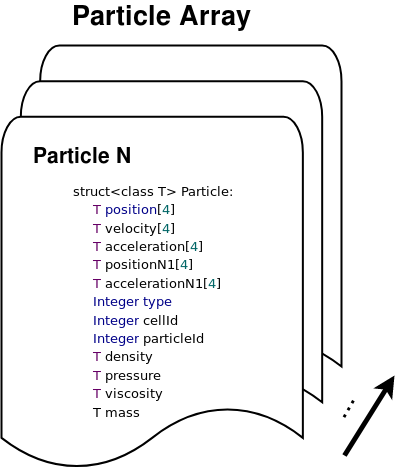
\includegraphics[scale=0.30]{p_struct}
  }
  \caption{Структура частицы.}\label{fig:p_struct}
\end{figure}

Таким образом модель описывается массивом частиц. При этом в зависимости от требования порядку точности вычислений можно варьировать обобщенный тип T между двумя интегральными типами данных \(float\) или \(double\). Каждая партиция определяется следующим образом пусть \(N\) – количество частиц \((p_0,...,p_{N-1})\) – упорядоченное по \(cellID\) множество начальных данных о частицах. Подразумевается, что каждый элемент \(p_i\) хранит пространственные координаты, координаты вектора скорости и \(cellID\) \(i\)-й частицы как показано на рисунке ~\ref{fig:p_struct}. Определим пространственные параметры модели 
\((x_{min}, y_{min}, z_{min})\), \((x_{max}, y_{max}, z_{max})\) – точки, определяющие границы области моделирования (вершины параллелепипеда, лежащие на его диагонали).
\(gridCellX\), \(gridCellY\), \(gridCellZ\)- количество пространственных ячеек по соответствующим измерениям трехмерного пространства. Эти значения получаются из целочисленного деления длины ребра ограничивающего объема на длину ребра пространсвенной ячейки например
\[
gridCellX = \left \lfloor \frac{\left |x_{max} - x_{min}  \right |}{2h} \right \rfloor
\]
\[
gridCellY = \left \lfloor \frac{\left |y_{max} - y_{min}  \right |}{2h} \right \rfloor
\]
\[
gridCellZ = \left \lfloor \frac{\left |z_{max} - z_{min}  \right |}{2h} \right \rfloor
\]
\(h\) – радиус сглаживания,
\(M\)– количество доступных устройств.

Для сравнительной оценки производительности устройства вводится эвристическая функция, которая рассчитывает коэффициент производительности на основе возможного количества потоков, которые можно одновременно запустить на конкретном устройстве:
\[
\epsilon(d_i)=D \cdot WG
\]
где \(d_i\) – устройство, \(D\)- количество доступных стриминговых мультипроцессоров (streaming multiprocessor - SM), для CPU – это число равно количеству ядер, \(WG\) – размерность рабочей группы для конкретного устройства. Например GPU Radeon R 290X обладает 44 стриминговых ядер, \(WG=256\).

Для достижения синхронности времени работы, необходимо, чтобы перед каждой итерацией данные были распределены между устройствами в количестве пропорциональном производительности устройств. Оптимальное количество частиц для обработки \(i\)-ым устройством определяется по следующей формуле:
\[
N_{i}^{'}=\left [ N \cdot \frac{\epsilon(d_i)}{\sum_{j}\epsilon(d_j)} \right ]
\]

Сформулируем еще два условия:
\noindent
\begin{enumerate}
  \item Все частицы, лежащие одной ячейке, должны обрабатываться одним устройством. Это условие можно сформулировать следующим образом:
\((C)\) \(\forall p_i, p_j\) \textit{если \(cellID\) частицы \(p_i=cellID\) частицы \(p_i\), то \(p_i, p_j\) обрабатываются одним устройством.}
  \item Количество пространственных ячеек обрабатываемых одним устройством должно быть кратным \(gridCellY\). 
\end{enumerate}

Следствием наложения этого условий является то, что итоговое количество частиц \(N_i \) для обработки \(i\)-м устройством  может отличаться от \(N_{i}^{'}\) (в зависимости от количества частиц в ячейке) т.е.:
\[
N_i = N_{i}^{'}+\Delta N_i, i=0,..., M-1 
\]
При этом:
\[
\sum_{j} N_j = \sum_{j}N_{j}^{'}=N
\]

Введем определение структуры партиции \(partition_i\) – структура для хранения индексов в общем массиве данных первой \(partition_{i}.start\) и следующей после последней частицы \(partition_{i}.end\), обрабатываемой \(i\)-м устройством с соблюдением условия 
\((C)\), которое достигается за счет упорядоченности множества частиц по номеру ячейки.  
\[
partition_{0}.start = 0
\]
\[
partition_{0}.end = partition_{0}.start + \epsilon (d_0) \cdot N + OFFSET_0 
\]
\[
...
\]
\[
partition_{i}.start = partition_{i-1}.end + 1
\]
\[
partition_{i}.end = partition_{i}.start + \epsilon (d_i) \cdot N + OFFSET_i, i=2,..., M - 1
\]
\(OFFSET_i\) – определяет количество частиц, которые находятся в добавочных ячейках (см. условие 2).
Заданные выше партиции определяют подмножества частиц, обрабатываемые соответствующими устройствами. Таким образом достигается распределение данных между устройствами так, что группы данных не пересекаются друг с другом. Как было уже сказано выше для корректности расчетов для частиц, которые находиться на границах партиций необходимо также учитывать частицы находящиеся в граничных ячейках соседних партиций.Устройство с номером  получает на обработку упорядоченный по  набор частиц. \fixme{К этому набору применяется параллельный метод PCI SPH. // тут нужно дописать}

\section{Модель вычислений.}\label{sec:ch3/sect2}

Модель вычислений определяет абстрактное представление того, как потоки инструкций выполняются в гетерогенной системе. Управляющая часть программы описывает, структуру, контролирующую ход вычислений и синхронизирует вычислительные узлы. Узел - отдельное независимое устройство GPU/CPU, обладающее изолированной памятью. В зависимости от количества узлов создается соответствующее количество параллельных потоков, выполняющих код отдельно, но в одном адресном пространстве. Каждый поток резервирует узел и контролирует вычисления на нем. Вычисления на узле могут проходить параллельно. Модель вычислений представлена на рисунке ~\ref{fig:calc1}.
\begin{figure}[ht]
  \centerfloat{
    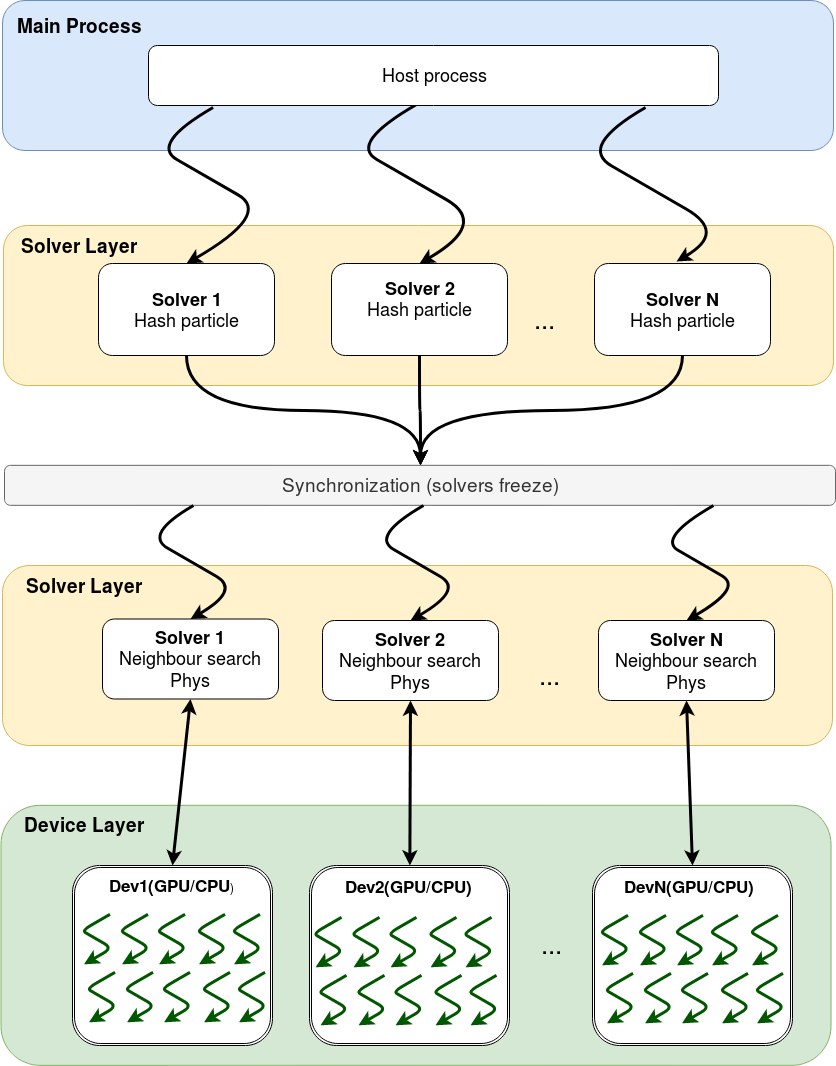
\includegraphics[scale=0.30]{calc1}
  }
  \caption{Модель вычислений.}\label{fig:calc1}
\end{figure}

Как видно из схемы, на этапе синхронизации все потоки  приостанавливаются, и хост-процесс синхронизирует данные, после чего вновь активирует их для дальнейшей работы. Синхронизация данных включает в себя процесс упорядочивания/сортировки массива частиц по соответствующему значению номера пространственной ячейки. Сортировка может работать в двух режимах: параллельном и \fixme{одно поточном}. При \fixme{одно поточном} режиме используется стандартная сортировка qsort \cite{Hoare1962}, сложность \(O(log(N))\). , реализованная в стандартной библиотеке шаблонов stl \cite{Stepanov1995} для языка C++ компилятора gcc. В параллельном режиме реализована модификация алгоритма цифровой сортировки \cite{Knuth1998}, минимизирующая количество перестановок частиц. ри этом вместо массива частиц строиться актуальная перестановка, при которой частицы упорядочены в  общем массиве. При этом процесс переупорядочивания также выполняется параллельно. За основу взята параллельная реализация радиксной сортировки \cite{Marcho1991}. На рисунке ~\ref{fig:sort1}. \fixme{показана схема работы процесса сортировки.}
\begin{figure}[ht]
  \centerfloat{
    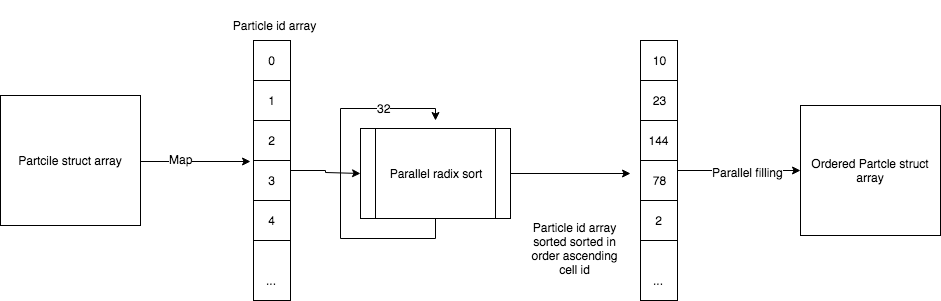
\includegraphics[scale=0.30]{sort1}
  }
  \caption{\fixme{...}}\label{fig:sort1}
\end{figure}

\section{Параллельная реализация в системе программирования OpenCL.}\label{sec:ch3/sect3}

...

\section{Результаты тестирования и оценки.}\label{sec:ch3/sect4}

...

















